% This is samplepaper.tex, a sample chapter demonstrating the
% LLNCS macro package for Springer Computer Science proceedings;
% Version 2.20 of 2017/10/04
%
\documentclass[runningheads]{llncs}
%
\usepackage{mathptmx}
\usepackage[T1]{fontenc}
% T1 fonts will be used to generate the final print and online PDFs,
% so please use T1 fonts in your manuscript whenever possible.
% Other font encondings may result in incorrect characters.
%
\usepackage{amsmath, amssymb}
\usepackage{graphicx}

% PDF Links --------------------------------------------------------
 \usepackage[colorlinks]{hyperref}
  \hypersetup{
    colorlinks=true, %
    linkcolor=black, %
    anchorcolor=black, %
    citecolor=black, %
    filecolor=black, % Color for URLs which open local files.
    menucolor=black, % Color for Acrobat menu items.
    urlcolor=black, %
    pdftitle={}, %
    pdfauthor={}, %
    pdfsubject={}, %
    pdfkeywords={}%
  }
\usepackage[]{cleveref}
\usepackage{microtype}
\usepackage{newtxtext,newtxmath}
\usepackage{siunitx}
\usepackage[numbers]{natbib}
\usepackage{booktabs}
\usepackage{gensymb}
\usepackage{url}
\usepackage{booktabs}
\usepackage{pifont}
\usepackage{glossaries}  

\usepackage{lscape}
\usepackage{geometry}
\geometry{
  left=1.5in,
  right=1.5in,
  top=1.5in,
  bottom=1.5in
}


\usepackage{scalerel,scalefnt}

\usepackage{tikz}
\usetikzlibrary{shapes.geometric, arrows, positioning}
% Define styles for the flowchart
\tikzstyle{block} = [rectangle, minimum width=4cm, minimum height=1cm, text centered, draw=black, fill=gray!10]
\tikzstyle{arrow} = [thick,->,>=stealth]



\usepackage{nomencl}
\setlength{\nomitemsep}{-\parsep}
\makenomenclature

\renewcommand{\nomname}{Nomenclature}
\renewcommand*{\nomlabel}[1]{#1}
\renewcommand{\thenomenclature}{%
    \section*{\nomname} % Adds non-numbered section-like heading
    \nompreamble % If you have any preamble text for the nomenclature
    \if@nomentbl
        \nompreamble
        \begin{longtable}{@{}p{0.3\linewidth}p{0.8\linewidth}@{}}
    \else
        \list{}{%
            %\labelwidth\nom@tempdim
            \leftmargin\labelwidth
            \advance\leftmargin\labelsep
            \itemsep\nomitemsep
            \let\makelabel\nomlabel
        }
    \fi
}



\begin{document}
%
\title{3D Heat Transfer Analysis in Architectural Modeling: A Case Study with OpenFOAM}
\titlerunning{3D Heat Transfer Analysis in Architectural Modeling}

%
% \author{Maryam Almaian\inst{1}\orcidID{0000-1111-2222-3333}, \\
% Patrick Kastner\inst{1}\orcidID{1111-2222-3333-4444}}

\author{Maryam Almaian, Patrick Kastner}


%\authorrunning{Almaian, M. et al.}
% First names are abbreviated in the running head.
% If there are more than two authors, 'et al.' is used.

\institute{School of Architecture, Georgia Institute of Technology\\ 
\email{\{malmaian3,pkastner3\}@gatech.edu}}
%
\maketitle              % typeset the header of the contribution
%

\vspace{-2\baselineskip}
\begin{abstract}
As global initiatives increasingly focus on sustainable building practices, architects are tasked with designing structures that not only fulfill aesthetic and functional requirements, but also minimize energy consumption. One critical aspect of achieving energy-efficient buildings is the selection of appropriate building materials to reduce heat loss through the building envelope.
The tools and software to simulate 2D/3D heat transfer are available, but often with limited features and are cost-prohibitive. The limitations of 2D heat transfer are the inability to simulate and explore complex geometry, corners, and the full analysis of the building envelope.
The integration of 3D thermal performance analysis into the architectural design process is an even more complex and underdeveloped area. 
This research aims to address this gap by exploring the use of OpenFOAM to simulate the ISO 10211:2007 A.3 heat transfer validation case.
%The outcomes of this paper aim to empower architects to make informed decisions about material selection and their impact on energy efficiency, by seamlessly embedding them into the Rhinoceros \& Grasshopper CAD environment. 

\keywords{
3D Heat Transfer  \and 
OpenFOAM 2306\and 
Conjugate Heat Transfer \and
Thermal Bridging \and
Rhinoceros \& Grasshopper   \and 
Parametric Architecture
}
\end{abstract}
%



\section{Introduction}
Climate change is one of the most significant challenges of our time and has severe consequences for the environment, society, and economy. The alarming increase in global land temperature, which has increased by approximately 40\% \cite{glb} recently, highlights the importance of addressing this issue. At the same time, buildings are major contributors to carbon emissions, emitting approximately 40 gigatons of $CO_2$ from operational carbon annually. To maintain the limit of global warming of 1.5 °C, it is necessary to reduce emissions by 10 gigatons of $CO_2$ per year, which is not feasible in current ASHRAE standards to comply with the minimum required insulation according to the location of a project. 

In adhering to these standards, there is a potential to optimize the selection of building materials to reduce heat losses and increase thermal comfort. Despite these recommendations, the process of modeling 3D heat transfer in buildings is a complex and long process due to the lack of free software available. This research aims to lay the foundations for providing architects with an easy-to-use 3D heat transfer workflow that, in the future, will be able to be integrated into architect design software, such as Rhino\, \&\, Grasshopper. Here, we used OpenFOAM (OF) / Grasshopper (GH) to construct an envelope segment from \textit{ISO 10211:2007 A.3}
\cite{ISO}, then calculate heat transfer and assess whether the validated case complies with our results. 

The research question is the following: (1) What approaches can be used to design and validate a workflow that simulates 3D heat transfer in architectural contexts? (2) How can this workflow be seamlessly integrated into existing architectural modeling software? These questions aim to bridge the gap in current simulation technology by investigating the creation of a more advanced and reliable 3D simulation solution for architectural projects.
%\clearpage
% -------------------------------------------------------
\section{Literature Review}
Current tools are often limited to 2D heat transfer, such as HTflux \cite{HTflux}, which is specialized software for simulations of two-dimensional heat and water vapor transport.
It uses the 2D Glaser method \cite{glaser1959graphisches} to calculate dew points, condensation, and evaporation in 2D structures. 
The software offers an easy-to-use interface, can import CAD geometries, and uses a direct mapping method for accurate simulations. 
It provides various thermal analysis metrics (heat flow, U-value, $\psi$-value, etc.) and measures extreme temperature values. Two contributions stand out that discuss different 3D heat transfer elements and approaches by \citeauthor{Yang} \cite{Yang} and \citeauthor{COMSOL} \cite{COMSOL}, while another contribution presents 2D heat transfer using OF \cite{kastner2020solving}.

\citeauthor{kastner2020solving} \cite{kastner2020solving} presented a case study that presents a thermal bridge analysis and 2D heat transfer with OF, which is similar to our approach due to the use of OF. The simulation is constructed from pre-processing, simulation, and post-processing. 
Based on the result of the used case, it is possible to use Rhino\ \&\ Grasshopper to calculate architectural heat transfer in the pre-and post-processing phases, but this requires additional research to achieve this goal. 
The authors experimented with a validation case retrieved from HTflux that was originally published in the ISO guide. 

The second approach is by \citeauthor{Yang} \cite{Yang} which experimented with 3D heat transfer following a different method, which is to develop a mesh using lumped hexahedral elements and employing ray/triangle intersection techniques for an accurate geometric representation of the building. 
It applies an energy balance to each element and integrates a system of ordinary differential equations to obtain spatio-temporal indoor temperature and relative humidity fields. 
However, there are several limitations, such as the inability to explicitly solve flow fields, which may limit its accuracy in capturing complex airflow patterns. 
Furthermore, idealized thermal conditions do not include real-world conditions and do not accurately represent the impact of the thermal mass of the floor. A summary table of the prominent tools and software for calculating heat transfer is illustrated in \Cref{tab:heat_transfer_software}.



\scriptsize
\begin{table}[htb]
    \centering
    \caption{Heat Transfer Simulation Software Overview.}
    \label{tab:heat_transfer_software}
    \hspace{-3.6cm}
    \scalebox{0.73}{
    \begin{minipage}[b]{1\textwidth}
    \begin{tabular}{ll>{\raggedright}p{4.5cm}lp{1cm}p{1cm}p{1.5cm}p{1cm}>{\raggedright}p{4cm}r} 
        \toprule
        Software & Type & Overview & Price & Rhino / Revit & Ease of Use & Complex Geometry & Export PV & Limitations & Source \\
        \midrule
        THERM     & 2D & Finite-element approach for complex geometries & \$0 & \ding{55} & \ding{51} & \ding{55} & \ding{55} & Limited to 2D, requires additional tools. & \cite{THERM} \\
        HTFLUX    & 2D & Heat and water vapor transport simulation & \$421/yr & \ding{55} & \ding{51} & \ding{55} & \ding{55} & Requires additional tool downloads. & \cite{HTflux} \\
        ENERGY2D  & 2D & Multiphysics including conduction, convection, and radiation & \$0 & \ding{55} & \ding{55} & \ding{55} & \ding{55} & No user interface. Requires additional tool downloads. & \cite{energy2d} \\
        HEAT2     & 2D & Transient and steady-state heat transfer & \$800/yr & \ding{55} & \ding{51} & \ding{55} & \ding{55} & Requires additional tool downloads. & \cite{heat2} \\
        Kelvin    & 2D & Temperature, heat flux, and gradient simulation & NA & \ding{55} & \ding{51} & \ding{55} & \ding{55} & Requires additional tool downloads. & \cite{kelvin} \\
        Quickfield & 3D & Static and transient heat transfer analysis & Node-based & \ding{55} & \ding{51} & \ding{51} & \ding{55} & Limited post-processing, additional tools. & \cite{quickfield} \\
        Simscale  & 3D & Models heat transfer in solids and fluids through convection & Core-based & \ding{55} & \ding{55} & \ding{51} & \ding{55} & Cost-prohibitive, limited post-processing. & \cite{simscale} \\
        COMSOL    & 3D & Heat transfer by conduction, convection, and radiation & \$4000 & \ding{55} & \ding{55} & \ding{51} & \ding{55} & Cost-prohibitive, requires additional tools. & \cite{COMSOL} \\
        theseus   & 3D & FEM for steady-state and transient analysis & NA & \ding{55} & \ding{51} & \ding{51} & \ding{51} & Limited post-processing, cost-prohibitive. & \cite{theusus} \\
        Physibel (S)  & 3D & Examines entire buildings with 2D/3D components & \$2,359/yr & \ding{55} & \ding{55} & \ding{51} & \ding{55} & Cost-prohibitive, limited post-processing. & \cite{physibel} \\
        TAITHERM  & 3D & Simulates transient or steady-state heat transfer & NA & \ding{55} & \ding{51} & \ding{51} & \ding{55} & Cost-prohibitive, limited post-processing. & \cite{taitherm} \\
        \bottomrule
    \end{tabular}
    \end{minipage}
    }
\end{table}
\normalsize





\section{Methodology}



The manuscript presents a simulation based on conductive and convective heat transfer. 
Conductive heat transfer can be calculated using the heat diffusion equation \citep{bergman2011fundamentals}:
	
	\begin{equation} 
	\frac{\partial^2 T}{\partial x^2}+
	\frac{\partial^2 T}{\partial y^2}+
	\frac{\partial^2 T}{\partial z^2}+ 
	\frac{\dot{q}}{k}= \frac{1}{\alpha}\frac{\partial T}{\partial t} \text{, with } \alpha = \frac{k}{\rho c_p}\quad \\
	\end{equation}
	
	
	Here, $x,y,$ and $z$ are Cartesian coordinates, $\alpha$ is the thermal diffusivity, $\dot{q}$ is the energy generation rate per unit volume, and $c_p$ is the specific heat capacity. To calculate convective heat transfer, the formula used accounts for both advection (the movement of heat with the fluid flow) and diffusion (the spatial variation of temperature): 

\begin{equation}
    \frac{\partial T}{\partial t} + \mathbf{v} \cdot \nabla T = \alpha \nabla^2 T + \frac{\dot{q}}{k},
\end{equation}

where $\mathbf{v}$ is the velocity vector of the fluid, $\alpha$ is the thermal diffusivity, $\nabla$ stands for the gradient operator, $\nabla^2$ represents the Laplacian operator, $\dot{q}$ is the energy generation rate per unit volume, and $k$ is the thermal conductivity \citep{bergman2011fundamentals}. The first step in the methodology is to select a 3D validation case study to model in Rhino. Then, GH is used to create a script that bridges the gap between Rhinoceros (the architectural modeling software) and OF (the CFD software package). A detailed description of the workflow, the GH automation, and the OF solver is illustrated in the following sections. 

   









\footnotesize
\begin{table}[bth]
    \centering
    
    
    \begin{minipage}{.5\linewidth}
      \caption{Construction material properties taken from the demo example in \textit{QuickField} \cite{quickfield}.}
      \label{tab:construction_material_properties}
      \centering
        
        \begin{tabular}{clrrr}    
            \toprule   
            & Materials       & $k$ $\left[ \si[per-mode=fraction]{\watt\per\metre\per\kelvin} \right]$ & $c_p$   $\left[ \si[per-mode=fraction]{\joule\per\kilogram\per\kelvin}\right]$ & $\rho$  $\left[ \si[per-mode=fraction]{\kilogram\per\cubic\metre} \right]$   \\ 
            \midrule
            & Floor Slab        & 2.5                        & 1000                      & 2300               \\
            & Aerated Concrete  & 2.5                        & 1000                      & 2300               \\
            & Brick             & 0.7                        & 1060                       & 710               \\
            & Insulation        & 1                         & 1450                      & 35               \\
            & Plaster           & 1                         & 1000                      & 2300              \\
            \bottomrule
        \end{tabular}
    \end{minipage}%
    \begin{minipage}{.5\linewidth}
      \caption{Temperature boundary conditions.}
      \label{tab:boundary_conditions}
      \centering
        \footnotesize
        \begin{tabular}{llrr}    
            \toprule   
            & Boundary conditions          & $T$ $[\si{\degreeCelsius}]$           & BC type                   \\ 
            \midrule
            & Inside temp.  (1st floor)         & 20                          & fixedValue                \\
            & Inside temp.  (2nd floor)          & 15                          & fixedValue                \\
            & Outside temp.  & 0                          & fixedValue                \\ 
            \bottomrule
        \end{tabular}
    \end{minipage}
\vspace{-0.3cm}
\end{table}
\normalsize



    
\subsection{Case Study setup}

The selected case study was chosen from the International Organization for Standardization (ISO) \cite{ISO}. The case study is a validated 3D heat transfer case documented in \textit{ISO 10211:2007 A.3}\footnote{ISO 10211:2007---Thermal bridges in building construction. Validation of case A.3 \cite{ISO}.}. The geometry consists of two levels: a first floor and a second floor, separated by a floor slab and a plaster floor. The walls are composed of aerated concrete, insulation material, and brick.
A description of each material in the geometry can be found in \Cref{fig:order-of-executables} (a). Beyond \textit{ISO 10211:2007 A.3}, it is also documented in QuickField 6.6 (student version) where the properties, layers, and boundary conditions of the materials are accessible, which we exported to compare it with our method. 
The geometry of the case study was exported from \textit{QuickField} and then modeled in \textit{Rhinoceros} and subsequently exported as a mesh to be processed with OpenFOAM. 
The validation case was constructed in \textit{OpenFOAM} by creating the mesh and \textit{snappyHexMesh} files.  

\subsection{Solver Setup}


The solver used in this case is \textit{chtMultiRegionFoam} in OpenFOAM 2306 which is a solver capable of solving steady or transient fluid flow with solid heat conduction and conjugate heat transfer between regions, buoyancy effects, turbulence, reactions, and radiation modeling (not used in this study) \cite{cht}. 
A crucial aspect is identifying the thermal properties that will allow the solver to identify the thermal conductivity, density, and properties of the material and calculate the heat transfer accordingly.
The outdoor ambient temperature is set to 0°C.  
%The setup of temperature boundary conditions could be handled easier by taking advantage of the initial temperatures based on the location. 
A description of the material properties and boundary conditions can be found in \Cref{tab:construction_material_properties} and \ref{tab:boundary_conditions}. 


%\clearpage
\subsection{Simulation}
The goal is to solve heat transfer in solids and liquids between air regions and the selected geometry. Using the software \textit{QuickField}  to solve for 3D heat transfer showed some limitations where it does not consider the air regions. However, our approach using OpenFOAM includes the integration between air and solids to produce more holistic results regarding the relevant building physics. 

\enlargethispage{2\baselineskip}


\begin{figure}[tbh] 
\includegraphics[width=0.36\columnwidth]{Figures/validationcase.PNG}
\includegraphics[width=0.36\columnwidth]{Figures/conductive.png}
\hspace{0.7cm}
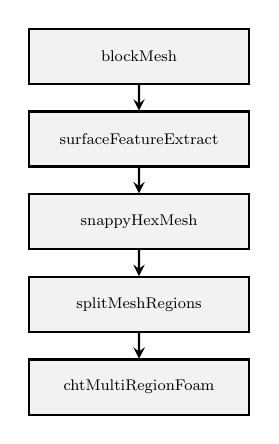
\begin{tikzpicture}[node distance=1.5cm, thick, scale=0.45, every node/.style={scale=0.7}]
% Define nodes
\footnotesize
\node (blockMesh) [block] {blockMesh};
\node (surfaceFeatureExtract) [block, below of=blockMesh] {surfaceFeatureExtract};
\node (snappyHexMesh) [block, below of=surfaceFeatureExtract] {snappyHexMesh};
\node (splitMeshRegions) [block, below of=snappyHexMesh] {splitMeshRegions};
\node (chtMultiRegionFoam) [block, below of=splitMeshRegions] {chtMultiRegionFoam};
% Connect nodes with arrows
\draw [arrow] (blockMesh) -- (surfaceFeatureExtract);
\draw [arrow] (surfaceFeatureExtract) -- (snappyHexMesh);
\draw [arrow] (snappyHexMesh) -- (splitMeshRegions);
\draw [arrow] (splitMeshRegions) -- (chtMultiRegionFoam);
\end{tikzpicture}

\hspace{2.6cm}(a)\hspace{4.9cm}(b)\hspace{4cm}(c)\hfill
\caption{validation geometry (a); vertical section of the validation case shows convection and conduction (b); Order of executables for multi region case setup with OpenFOAM v2306 (c).}
\label{fig:order-of-executables}
\vspace{-0.5cm}
\end{figure}






\Cref{fig:order-of-executables} illustrates the executables that need to be executed in order for a multiregion case.
The \textit{blockMesh} utility generates parametric meshes incorporating grading and curved edges. 
The meshes are created based on the specifications specified in a dictionary file named \textit{blockMeshDict}  within the case directory.
\textit{surfaceFeatureExtract} extracts the surface features and records them in a file.      
\textit{snappyHexMesh} is a utility in OpenFOAM that generates 3D meshes with hexahedra from STL surfaces, iteratively refining while maintaining surface conformity.
\textit{splitMeshRegions} divides the mesh into separate regions. Each region consists of cells that can be reached without crossing boundary faces, including cell zones.
\textit{chtMultiRegionFoam} is our chosen solver for steady and transient multiregion fluid flow, with solid heat conduction and conjugate heat transfer. The equations for each system variable are solved, and the solutions from preceding equations are inserted into the subsequent ones. For instance, fluid-solid coupling solves fluid equations first, using the previous iteration's solid temperature to set fluid temperature boundary conditions. The simulation using this process continued until convergence at time step 4,400.
    
\section{Results} 
\Cref{fig:paraview} (a) visualizes the simulation temperature output produced by OF, while \Cref{fig:paraview} (b) shows the Quickfield results. The magenta temperature probes are shown in the plot in \Cref{fig:validation-plots} which details the QuickField output and our OF simulation along the z-axis from $z= 1.2$ to $z=2.2\, \text{m}$. The magenta line shown in \Cref{fig:paraview} (a) represents a non-linear temperature gradient as a result of the different specific heat capacities and thermal conductivity of the materials. The peak at $z=1.8\, \text{m}$ refers to the temperature of the slab. 



\begin{figure}[tbh]
    \centering
    \begin{minipage}[b]{0.45\linewidth}
        \centering
        \textbf{(a)}\\
        \includegraphics[trim=5cm 0cm 4.5cm 0cm, clip, width=\linewidth]{Figures/newvalleg.pdf}
    \end{minipage}
    \hspace{0.5cm}  % Adjust the horizontal space between the images
    \begin{minipage}[b]{0.45\linewidth}
        \centering
        \textbf{(b)}\\
        \includegraphics[width=\linewidth]{Figures/ValidationCaseClean.png}
    \end{minipage}
    \caption{3D Validation Visualization: (a) OF case 3D results, (b) Quickfield validation results. The temperatures from the magenta probing line are shown in \Cref{fig:validation-plots}.}
    \label{fig:paraview}
\end{figure}



\begin{figure}[tbh] 
\centering
\includegraphics[trim= 2cm 0.2cm 1cm 1.5cm, clip= true, width=1\columnwidth]{Figures/valpl2.png}
\hspace{0.3cm}
\caption{Temperature gradients probed from the magenta line in \Cref{fig:paraview}  (a).}
\label{fig:validation-plots}
\end{figure}





%\clearpage
\section{Discussion}

The workflow presented in this paper can be considered an extension of work by \citeauthor{kastner2020solving} \cite{kastner2020solving}. The findings highlight several issues in the field, such as cost-prohibitive software and the disconnect between architectural modeling with heat transfer modeling software. 
The simulation focuses on convective and conductive heat transfer for a 3D heat transfer problem recognized as an international comparison case. The 3D validation case study consists of two-floor corner sections separated by a concrete slab with a balcony. This case study was selected because it has the potential to present many coupling challenges in heat transfer, such as 3D thermal bridges, as well as fluid/soid interactions.

Our results generally comply with the ISO guidelines. However, the differences shown in \Cref{fig:validation-plots} are due to the modeling approach used in Quickfield, where the slab is separated from the model, which we were unable to reproduce for this manuscript.
However, we are confident that this can be solved in a future iteration of this simulation approach. 
We gained this confidence through an additional validation effort for \textit{chtMultiRegionFoam}, where we carried out a physical experiment using heat flux sensors for a single-region brick wall, including a varying outdoor boundary condition in one of our academic buildings \cite{almaian2024heat}. In this experiment, we report a percentage of error that varies from 0.003 \% to 0.01 \% 


The overall results illustrate the capabilities of using Rhino and GH to simplify the pre-processing and post-processing steps to run the 3D heat transfer simulation in OF. 
We believe that the 3D heat transfer workflow can help improve decision-making in building performance by contributing to the selection of appropriate materials, analyzing thermal comfort, and optimizing insulation. %Thus, having an integrated 3D heat transfer workflow incorporated from the preliminary design phase to the schematic phase is essential to ultimately reduce the building's operational and embodied carbon emissions. 


\enlargethispage{2\baselineskip}


%\clearpage
\section{Conclusion}
This work presents an automated integration of Grasshopper, Rhinoceros, and OpenFOAM to simulate the ISO 10211:2007 A.3 thermal bridge validation case. Using OF, this automated 3D heat transfer modeling approach fills a critical gap in current design practices and can inform energy-efficient building design and data-driven material selection. Future work in this field should focus on packaging the GH automation workflow into a user-friendly plug-in. A plug-in would simplify the process of simulating 3D heat transfer for other modelers, allowing them not only to build the case and create the mesh, but also to run any OF simulations without the need to manually write text files. 

\enlargethispage{2\baselineskip}


\vspace{0.15in}
\small
\nomenclature{\(CHT\)}{Conjugate Heat Transfer}
\nomenclature{\(PCM\)}{Phase Changing Materials}
\nomenclature{\(CAD\)}{Computer-aided design}
%\nomenclature{\(ASHRAE\)}{American Society of Heating, Refrigerating and Air-Conditioning Engineers}
\nomenclature{\(C_p\)}{Specific heat capacity, \si{\joule\per\kilogram\per\kelvin}}
\nomenclature{\(d\)}{Length, \si{\metre}}
\nomenclature{\(h\)}{Heat transfer coefficient, \si{\watt\per\metre\squared\per\kelvin}}
\nomenclature{\(k\)}{Thermal conductivity, \si{\watt\per\metre\per\kelvin}}
\nomenclature{\(\Psi\)}{Linear thermal transm. coeff., \si{\watt\per\metre\per\kelvin}}
\nomenclature{\(GH\)}{Grasshopper}
\nomenclature{\(OF\)}{OpenFOAM}
\nomenclature{\(q\)}{Heat flux density, \si{\watt\per\metre\squared}}
\nomenclature{\(U\)}{Thermal transmittance, \si{\watt\per\metre\squared\per\kelvin}}
\nomenclature{\(T\)}{Temperature, \si{\celsius\kelvin}}
\nomenclature{\(x,\ y,\ z\)}{Cartesian coordinates, \si{\metre}}
\nomenclature{\(ASHRAE\)}{American Society of Heating, Refrigerating and Air-Conditioning Engineers}
\nomenclature{\(GH\)}{Grasshopper}




\vspace{0.15in}
\fbox{\parbox{0.88\columnwidth}{%
    \vspace{2mm}% Add top padding if desired
    \hspace{3mm}% Adjust the 5mm as needed for left padding
    \begin{minipage}{0.97\columnwidth}
        \printnomenclature
    \end{minipage}
    %\hspace{0mm}% Right padding
    \vspace{2mm}% Add bottom padding if desired
}}



\bibliographystyle{plainnat}
\bibliography{xbib}
% Print the nomenclature within a box with left padding

\end{document}